
\section{Results}
\label{sec:results}

We implemented the UCB-1 and $\epsilon$-Greedy bandits on each of the following distributions:

\begin{figure}[htb]
  \centering
  \begin{tabular}{|c|c|c|} 
    \hline \hline     
    Distribution & Machine  \\ 
    \hline 
     & 1 & 2 & 3 & 4 & 5 & 6 & 7 & 8 & 9 & 10 \\
    1 & 0.9 & 0.6 &  &  &  &  &  &  &  &  \\
    3 & 0.55 & 0.45 & 3 & 4 & 5 & 6 & 7 & 8 & 9 & 10 \\
    11 & 0.9 & 0.6 & 0.6 & 0.6 & 0.6 & 0.6 & 0.6 & 0.6 & 0.6 & 0.6 \\
    14 & 0.55 & 0.45 & 0.45 & 0.45 & 0.45 & 0.45 & 0.45 & 0.45 & 0.45 & 0.45 \\
    \hline \hline
  \end{tabular}
  \caption{The machines use Bernoulli reward distributions as allotted above.}
  \label{tab:Bernoulli Reward Distributions}
\end{figure}

\subsection{UCB1}
\label{subsec:UCB1}

Over $10^5$ runs, the UCB1 bandit produced the following results:

\begin{figure}[htb]
  \centering
  \begin{tabular}{|c|c|c|} 
    \hline \hline     Bandit & Percentage of Optimal Plays &  Cumulative Regret \\  using the &
    \hline 
     1 & 99.738 & 80.0 \\
     3 & 97.946 & 189.0 \\
     11 & 97.993 & 618.0 \\
     14 & 87.374 & 1330.0 \\
    \hline \hline
  \end{tabular}
  \label{tab:Statistics for UCB1 Bandits}
\end{figure}

We see that in every case, the bandits play the optimal machine very often in each case. As we can see in the figures below, the bandits converge of the optimal machine in logarithmic time:

\begin{figure}[htb]
  \centering 
  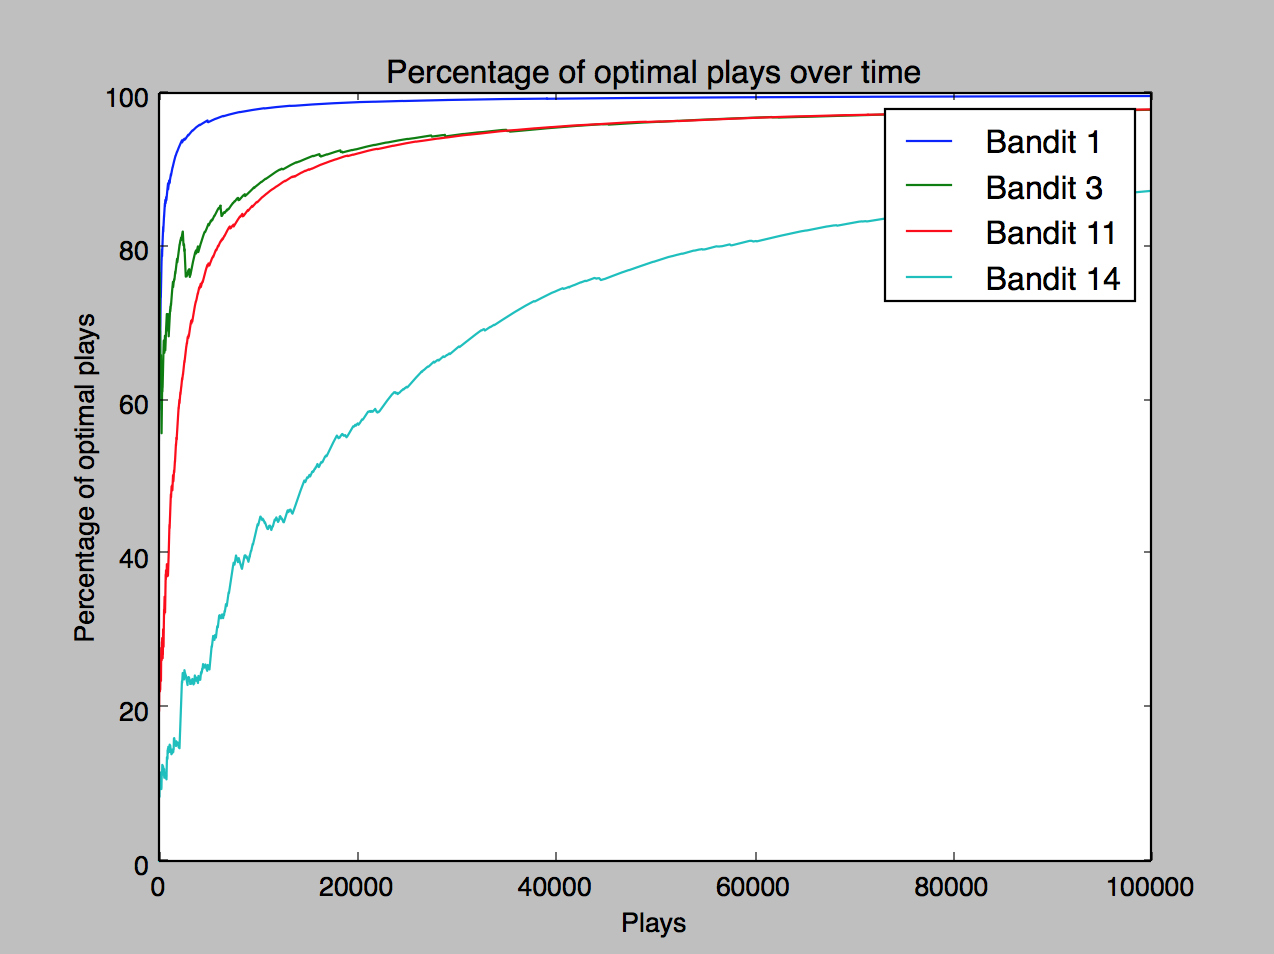
\includegraphics[width=0.47\textwidth]{ucb_plays_14.png}
  \caption{Graph of percentage of optimal plays over time for each UCB1 Bandit}
  \label{fig:UCB1 Percentage of optimal plays over time}
\end{figure}
\begin{figure}[htb]
  \centering 
  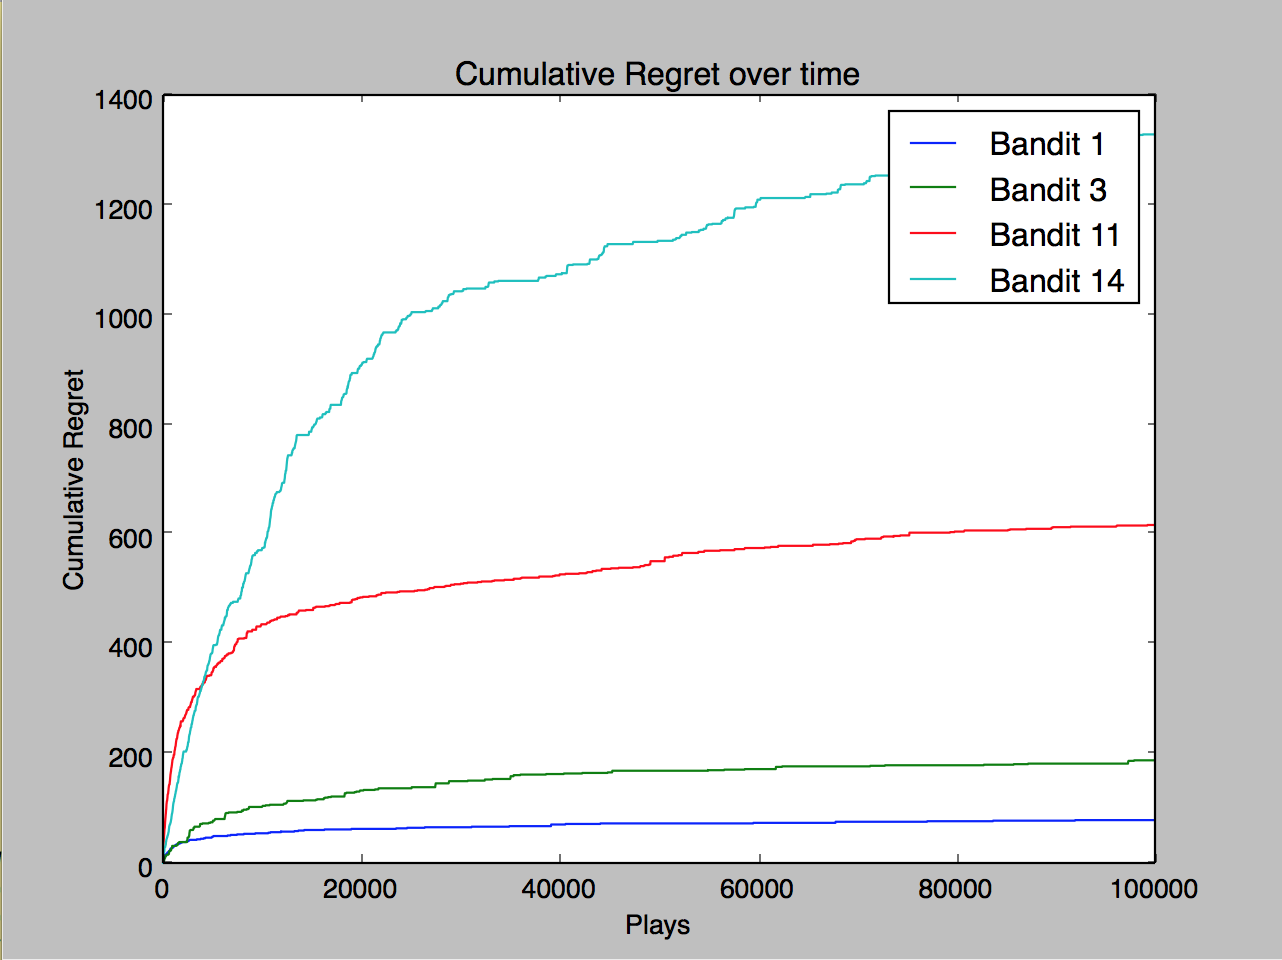
\includegraphics[width=0.47\textwidth]{ucb_regret_14.png}
  \caption{Graph of Cumulative Regret over time for each UCB1 Bandit}
  \label{fig:UCB1 Cumulative Regret over time}
\end{figure}

Bandit 1 and Bandit 2, the 2-armed bandits, reach a much lower maximum cumulative regret than bandits 11 and 14, the 10-armed bandits. We can see that as the bandit is given more machines to choose from, it takes longer to converge to the optimal machine. All four bandits played the best machine an overwhelming majority of the time, with bandits 1, 3, and 11 playing the optimal strategy over $97\%$ of the time, while Bandit 14 came in just under $90\%$ at around $87\%$.

These results show that the UCB1 bandit algorithm works very quickly on reward distributions with fewer machines, but takes longer as the number of machines, n, increases.

\subsection{$\epsilon_n$-greedy}
\label{subsec:$\epsilon_n$-greedy}

The $\epsilon$-greedy algorithm converged very quickly to the optimal machine. Over 10^5 runs, the bandit produced the following results:

\begin{figure}[htb]
  \centering
  \begin{tabular}{|c|c|c|} 
    \hline \hline 
    Bandit & Percentage of Optimal Plays &  Cumulative Regret \\ 
    \hline 
     1 & 99.839 & 360.0 \\
     3 & 99.818 & 374.0 \\
     11 & 98.675 & 1481.0 \\
     14 & 88.660 & 1505.0 \\
    \hline \hline
  \end{tabular}
  \label{tab:Statistics for $\epsilon_n$-greedy Bandits}
\end{figure}

\begin{figure}[htb]
  \centering 
  \includegraphics[width=0.47\textwidth]{e_greedy_play.png}
  \caption{Graph of percentage of optimal plays over time for each $\epsilon_n$-greedy Bandit}
  \label{fig:$\epsilon_n$-greedy Percentage of optimal plays over time}
\end{figure}
\begin{figure}[htb]
  \centering 
  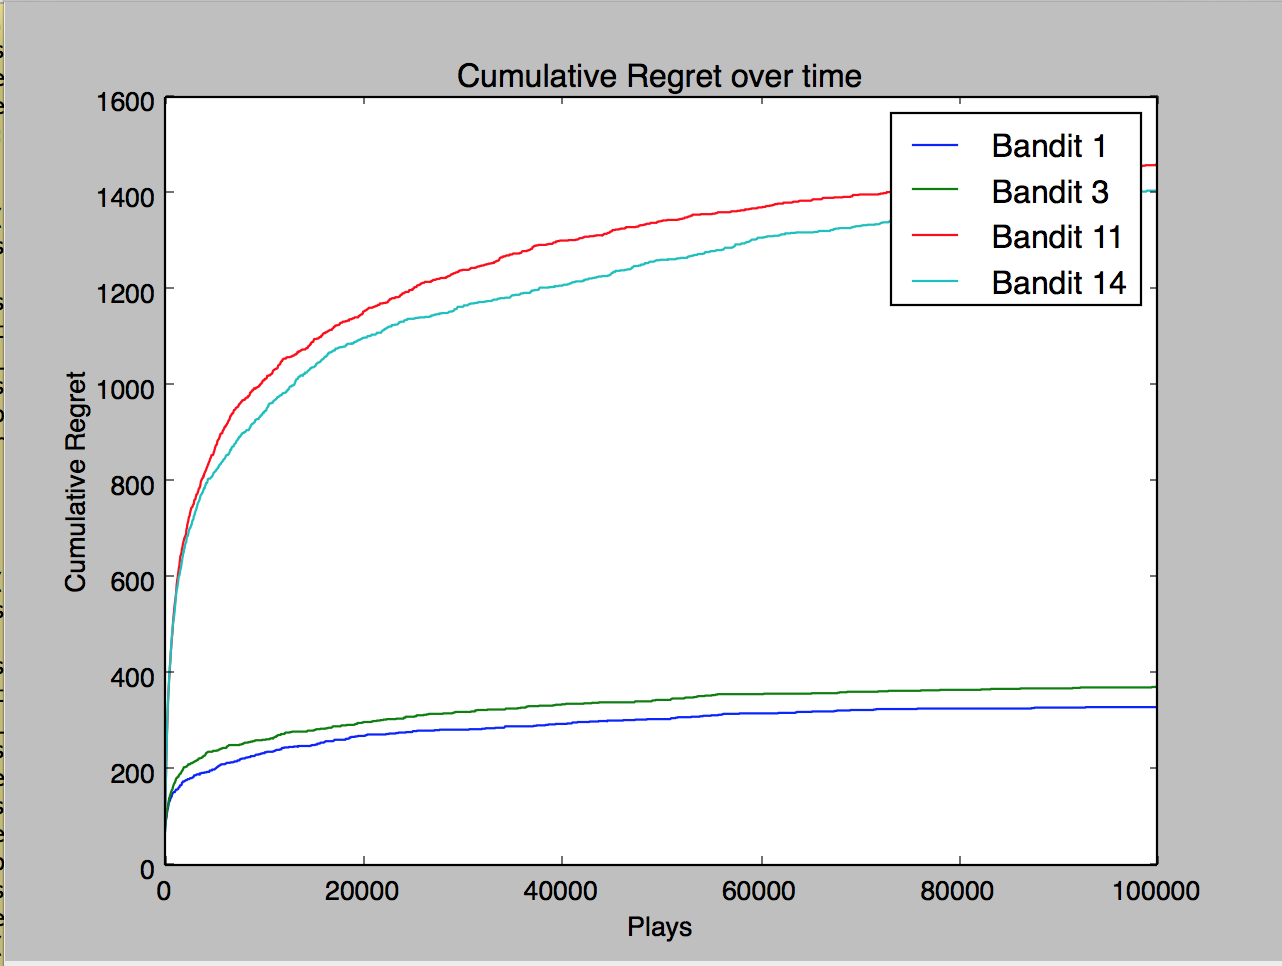
\includegraphics[width=0.47\textwidth]{e_greedy_regret.png}
  \caption{Graph of Cumulative Regret over time for each $\epsilon_n$-greedy Bandit}
  \label{fig:$\epsilon_n$-greedy Cumulative Regret over time}
\end{figure}

We see that in every case, the bandit played the optimal machine the overwhelming majority of the time. The cumulative regret is higher for bandits 11 and 14, as those had 10 machines to choose from, and thus took longer to converge to the correct machine. However, as we see from the graphs, the bandits did converge to the optimal machine and played it better than 98 percent of the time. By decreasing the value of $c$, we can achieve nearly perfect results. Auer et. al. tested values  of $c = 0.15, 0.10,$ and $0.05$. We replicated these results, and saw that the smallest $c$ values lead to outstanding results. The following were produced with $c = 0.05$:
\begin{figure}[htb]
  \centering
  \begin{tabular}{|c|c|c|} 
    \hline \hline 
    Bandit & Percentage of Optimal Plays &  Cumulative Regret \\ 
    \hline 
     1 & 99.999 & 3.0 \\
     3 & 99.998 & 5.0 \\
     11 & 98.976  & 26.0 \\
     14 & 98.980 & 23.0 \\
    \hline \hline
  \end{tabular}
  \label{tab:Statistics for $\epsilon_n$-greedy Bandits with $c = 0.5$}
\end{figure}

\begin{figure}[htb]
  \centering 
  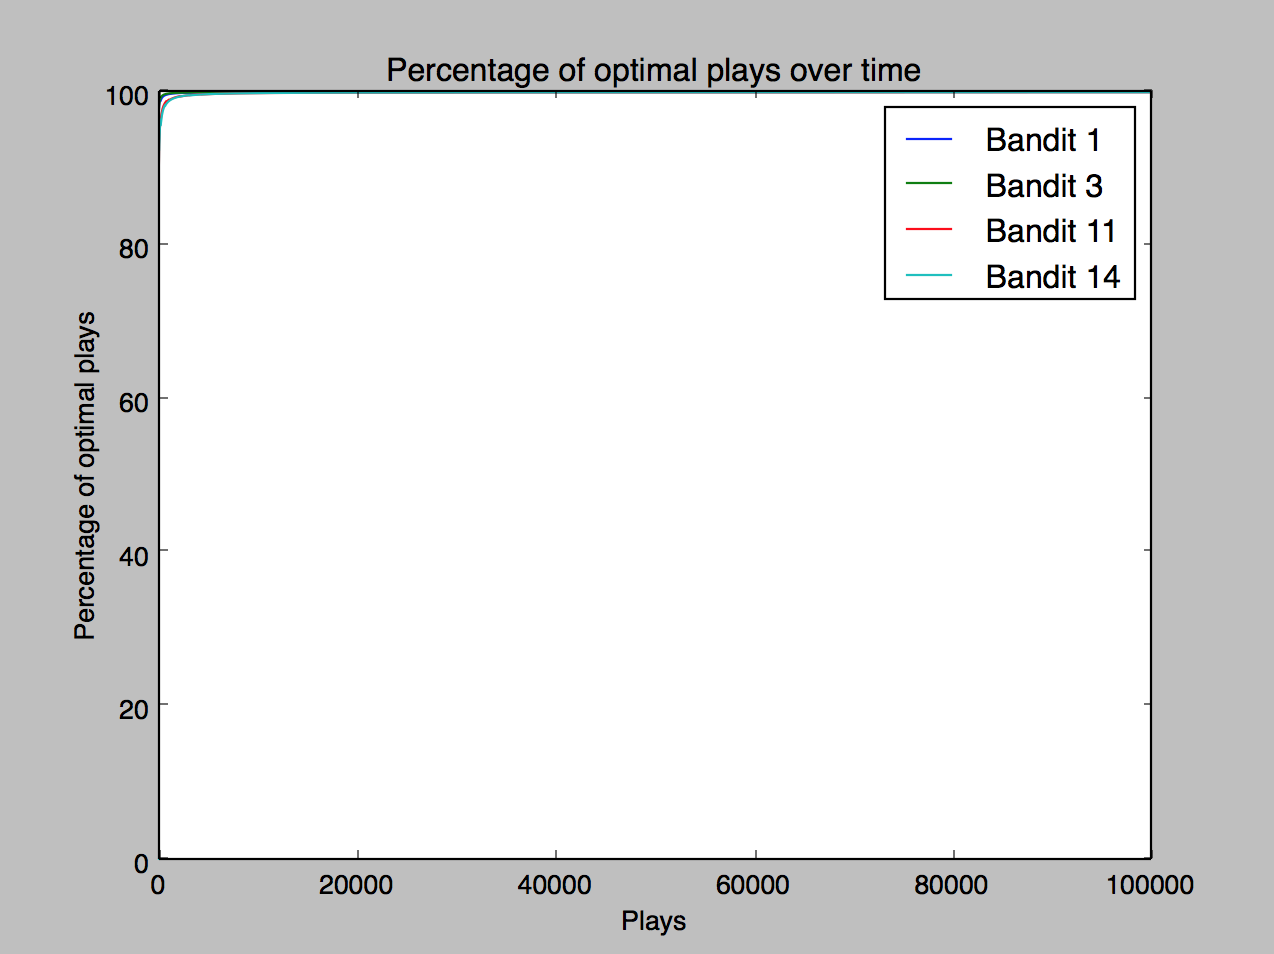
\includegraphics[width=0.47\textwidth]{plays_c_05.png}
  \caption{Graph of percentage of optimal plays over time for each $\epsilon_n$-greedy Bandit with $c = 0.5$}
  \label{fig:$\epsilon_n$-greedy Percentage of optimal plays over time ($c = 0.5$)}
\end{figure}
\begin{figure}[htb]
  \centering 
  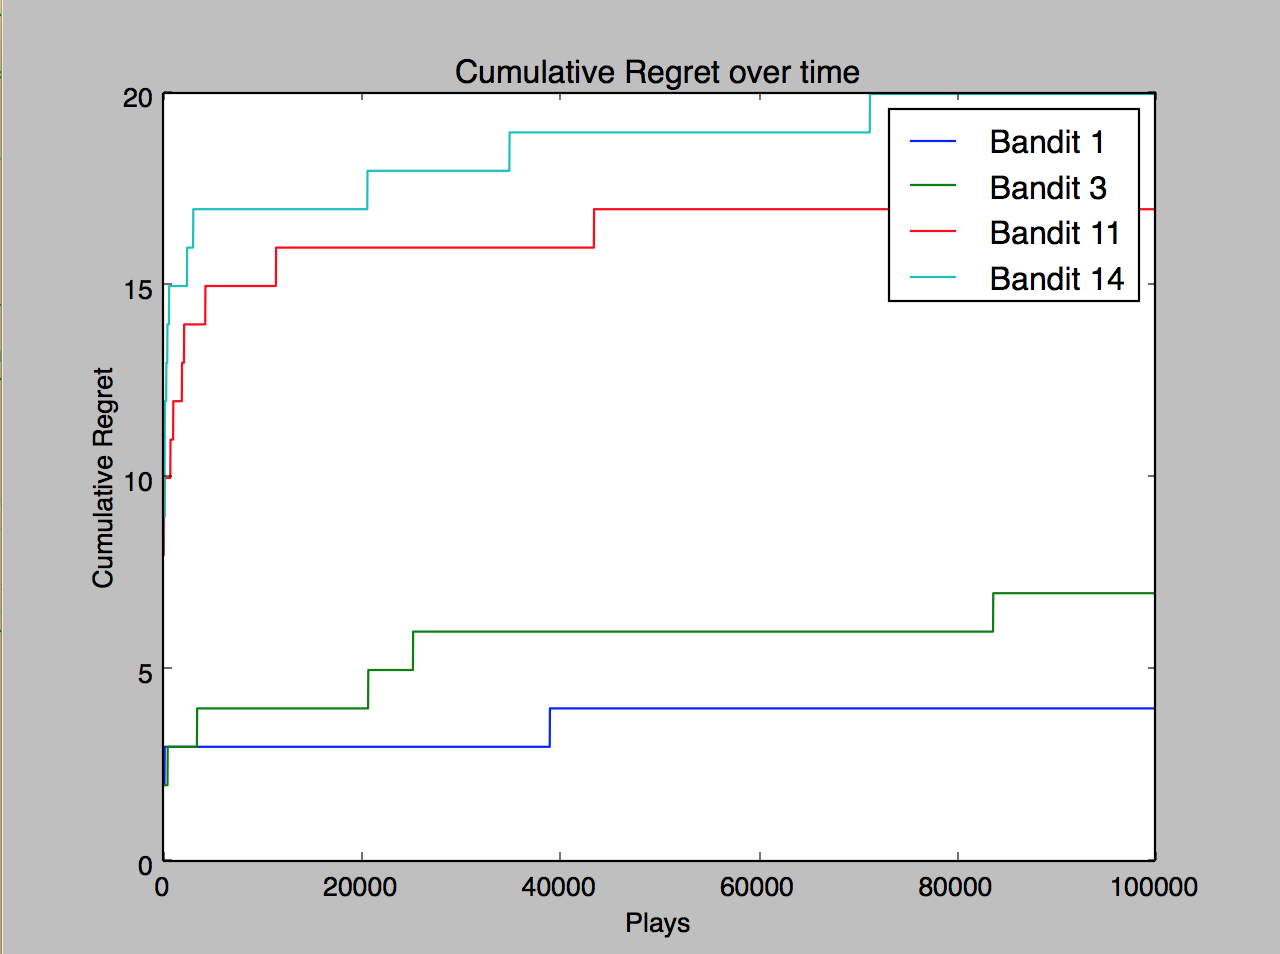
\includegraphics[width=0.47\textwidth]{regret_c_05.png}
  \caption{Graph of Cumulative Regret over time for each $\epsilon_n$-greedy Bandit with $c = 0.5$}
  \label{fig:$\epsilon_n$-greedy Cumulative Regret over time ($c = 0.5$)}
\end{figure}

These results clearly demonstrate a near-perfect playing strategy with a small c value.

In both the UCB-1 and $\epsilon$-Greedy cases, we see that Bandits 3 and 14 had a harder time converging than Bandits 1 and 11. This is due to the underlying distributions being played. Bandits 1 and 11 played distributions with a clear best choice, while 3 and 14 had much more uniform choices to choose from. This made it harder to determine which was the best choice, but ultimately both algorithms were able to do so. We found that the most effective strategy for approaching the multi-armed bandit problem, between these two algorithm, is to use the $\espilon_n$-greedy algorithm with a small $c$-value

